\documentclass[12pt, twoside]{report}
\usepackage{babel}
\usepackage[a4paper,width=150mm,top=25mm,bottom=25mm]{geometry}
\sloppy 
\usepackage{graphicx}
\graphicspath{ {assets/} }
\usepackage{titlesec}

\titleformat{\chapter}{\normalfont\huge}{\thechapter.}{20pt}{\huge}

\title{
	{\large \textbf {Szegedi Tudományegyetem}}\\
	{\large \textbf {Informatikai Intézet}}\\
	\textbf {Keresztplatformos alkalmazás fejlesztése nagy fájlok kezelésére felhőbe}\\
	{\large (Development of a cross-platform application for handling large files in the cloud)}\\
	{Szakdolgozat}\\
	{\small Készítette:}\\
	\textbf {\large Fodor Beáta}\\
	{\small Témavezető:}\\
	\textbf {\large Dr. Bilicki Vilmos}\\
	{Szeged}\\
	{2021}\\
}
\date{}

\begin{document}

\maketitle
\newpage

\chapter*{Feladatkiírás}
Szakdolgozatom célja egy felhő alapú, általános fájlkezelő mobilalkalmazás létrehozása volt, amely képes kezelni a nagyméretű fájlokat, emellett a feltöltés és a már feltöltött fájlok elérése valós időben történjen. Mindezt, elsősorban Android és iOS pluginok, továbbá a Firebase SDK használatával.

\chapter*{Tartalmi összefoglaló}


\chapter*{Tartalomjegyzék}


\chapter*{Motiváció}
Az utóbbi években, a modernizációnak és a gépiesedésnek köszönhetően, egyre több adat érhető el elektronikusan. Az elektronikus tárolás mind, akár a környezetünk védelmét, mind a saját kényelmünket szolgálja. De a különböző technológiák, hihetetlen mértékű és gyorsaságú fejlődése ellenére is, szükségünk van ezeknek az adatoknak egy, úgynevezett biztonsági mentésére is. Emiatt, és azért, hogy ezeket az adatokat akármikor, bármilyen eszközről, szinte azonnal elérhessük, fejlesztették ki a felhő alapú szolgáltatásokat.
Szakdolgozatom célja egy olyan alkalmazás fejlesztése volt, amely a fájlok felhőben való tárolását, és a már feltöltött fájlok kezelését, továbbítását valósítja meg mobileszközökön. A következőkben, először a felhő alapú szolgáltatások lényegét és alapvető működését, majd az általam készített szoftvert, azon belül is annak működését, használatát, alkalmazott technológiáit mutatom be.

\chapter{Betekintés a felhő-számítástechnikába}
\section{Mi a felhő-számítástechnika?}
A felhő-számítástechnika a különböző számítási szolgáltatások, mint például az adatbázis kezelés, tárolás, elemzés interneten keresztüli elérhetővé tétele az úgynevezett felhőben. Ezek a felhőalapú szolgáltatások a lokális megvalósításnál rugalmasabbak, idő- és méretgazdaságosabbak, ezáltal költséghatékonyabbak, internetkapcsolat birtokában pedig szinte azonnal elérhetőek.\\
Legnagyobb előnye, hogy megkíméli a felhasználót ezeknek a szolgáltatásoknak a futtatásához szükséges hardveres- és szoftveres erőforrásoknak és igényeiknek a költségeitől. Ezek mind a használt felhőszolgáltató birtokában állnak, melyeket ők bocsájtanak a felhasználók részére. A felhőszolgáltatók igyekeznek ezeket az erőforrásokat a legújabb és legmegbízhatóbb hardvereszközök működtetésével biztosítani, ezáltal a szolgáltatások pillanatok alatt eleget tesznek a felhasználó által indított kérésnek.

\section{Felhő-számítástechnika alkalmazásai}
Ma már a legtöbb online szolgáltatás mögött a felhő-számítástechnikai háttér áll. Kis- és nagyvállalatok, közigazgatási- és non-profit szervezetek legkülönbözőbb szolgáltatásai egyaránt épülhetnek felhőalapú szolgáltatásokra. Ezek lehetnek adtat tárolást, hang- és/vagy videótartalom streamelését, adatok elemzését, intelligencia beágyazását megvalósító szolgáltatások, vagy saját natív felhőalkalmazások is.

\section{Felhő-szolgáltatások típusai}
Az úgynevezett felhő-számítástechnikai halomba négy, egymásra épülő kategória tartozik. A felhőszolgáltatások a felhasználói igények függvényében különbözőek lehetnek, többségét a négy kategória valamelyikébe lehet sorolni.
\subsection{Infrastruktúra-szolgáltatás (IaaS)}
Ebbe az esetben egy azonnal elérhető számítástechnikai infrastruktúrát áll rendelkezésre, mely üzembe helyezése és felügyelése az interneten keresztül történik. Az igénybevevő mentesül a szerverek megvásárlásának és üzemeltetésének tényleges költségei, feladatai alól. Ezt a szolgáltató nyújtja számára, általában használatalapú díjfizetés ellenében, és minden szolgáltatás külön, mintegy szolgáltatás-összetevőként vehető igénybe.
\subsection{Platformszolgáltatás (PaaS)}
Az úgynevezett platformszolgáltatás már nem csak az üzem behelyezési, de a teljes körű fejlesztési környezetet is biztosítja az igénybevevő számára. Az infrastruktúra-szolgáltatáshoz hasonlóan a platformszolgáltatás is tartalmazza az infrastruktúrát (tárhely, kiszolgálók, hálózat), de emellett a fejlesztőeszközöket, adatbázis-kezelő rendszereket, közbenső szoftvereket és hasonlókat is kínál. Mindezek segítségével egy teljes web alkalmazás fejlesztését és üzemeltetését teszi lehetővé. Legfőbb előnyei közé tartoznak például a fejlesztés gyorsítása, földrajzi korlátainak áthidalása és a többplatformos alkalmazások létrehozásának megkönnyítése.
\subsection{Kiszolgáló nélküli számítástechnika}
Ez egy, a platformszolgáltatást átfedő szolgáltatások csoportja, mely lehetővé teszi, hogy a fejlesztő mentesüljön az infrastruktúra kezelése alól, ezek számára láthatatlanok. Az infrastruktúra kiépítését, méretezését és kezelését a felhőszolgáltató végzi el helyette, de a kódot továbbra is a kiszolgáló futtatja. Előnye, hogy meggyorsítja a fejlesztést és a termék piacra kerülését.
\subsection{Szoftverszolgáltatás (SaaS)}
A szoftverszolgáltatás, a négy kategória közül, áll a legközelebb az átlag felhasználóhoz. Felhőalapú szolgáltatásokhoz való kapcsolódását és használatát teszi lehetővé az interneten keresztül. Az igénybevevő már egy kész szoftvert használ, amely a háttérben implementálja a felhőszolgáltatások minden előnyét. Általában használatalapú díjfizetés ellenében a felhőszolgáltató rendelkezésre bocsájtja a használni kívánt szoftvert, ami lehet például egy e-mail vagy különböző irodai eszközök szoftvere is, melyeket web böngészőn keresztül ér el és használ. A szolgáltató birtokolja, üzemelteti és felügyeli az infrastruktúrát, a közbenső szoftvereket és magát az alkalmazást is, az igénybevevőnek csak használnia kell azt.


\chapter{Meglévő felhőalapú tároló alkalmazások}
Ma már rengeteg alkalmazás létezik a fájlok felhőben való tárolására, akár biztonsági mentésként szeretnénk használni, akár azért, hogy a különböző eszközeinken is mindig elérjük őket, vagy éppen azért, hogy másokkal megosszuk őket. A legnépszerűbbek a nagyvállalatok szolgáltatásai, de ha éppen nem szeretné valaki tartósan tárolni ezeket a fájlokat, akkor akár regisztráció nélkül a kisebb szolgáltatók alkalmazások is hasznosak lehetnek. Az alábbiakban a legnépszerűbb felhőalapú tároló alkalmazásokat mutatom be.

\section{GoogleDrive}
A Google által fájlok tárolására, szinkronizálására és szerkesztésére fejlesztett szoftver. Az alkalmazásban regisztrációt követően a hozzáférünk saját felhőalapú tárhelyünkhöz, ahová feltölthetjük fájljainkat és könyvtárainkat, szerkeszthetjük, megoszthatjuk őket.
A tárhelyünket a webes felületen vagy az alkalmazáson való bejelentkezés után bármely web böngészőből, Windows (XP+), Android (2.1+) vagy iOS (3.0+) eszközről elérhetjük.

\section{Dropbox}
A Dropbox Inc. által fejlesztett fájltárolási és szinkronizálási szolgáltatása. Használatával egy közös könyvtár segítségével a felhasználó különböző eszközei kapcsolhatók össze, az itt történő változások automatikusan szinkronizálódnak ezeken az eszközökön, továbbá megoszthatóak más felhasználókkal.\\
Az alkalmazás elérhető bármelyik böngészőből, Windows, macOS, Linux asztali-, valamint a legtöbb mobil operációsrendszer (Android, iOS, BlackBerry OS, Symbian, Windows Phone) áruházából letölthető alkalmazásain.

\section{OneDrive}
Vagy más néven SkyDrive, a Microsoft saját fejlesztésű felhőalapú fájlokat tároló, megosztó és szinkronizáló szoftvere. Windows rendszereken nem csak fájlok, de a felhasználói rendszerbeállítások tárolására is alkalmas. Elérhető web böngészőn keresztül, mobil eszközökön (Android, iOS, Windows Phone), Windows és macOs asztali alkalmazások használatával, továbbá Xbox 360, One, Series S és Series X konzolokon is.

\section{MediaFire}
Egy, a MediaFire saját fejlesztésű fájlok tárolására, szinkronizálására és megosztására használható alkalmazása. A felhasználó a web böngészőn túl, Windows, macOS, Linux asztali-, valamint Android, iOS és BlackBerry 10 mobil alkalmazásain is elérheti a tárhelyét és az oda feltöltött fájljait.

\section{Összegzés}
A fent felsoroltak mindegyike egy jól használható, egy adott tárhely méretig ingyenes, ami a felhasználói igényeknek megfelelően bővíthető, a legtöbb manapság használt platformon elérhető, nagy népszerűségnek örvendő szoftverek. Az alapvető fájlkezelés, mint a fájlok átnevezése, törlése, a feltöltött fájlok listázása, letöltése és megosztása alapfunkciók. A tárhelybe feltölthetők egy vagy egyszerre akár több fájl, könyvtárak, valamint kezelik a nagyméretű fájlokat is. A feltöltési folyamat szintén mindegyik alkalmazás esetében megszakítható, viszont a feltöltést újrakezdeni nem tudjuk. Ez a kisebb fájloknál általában nem okoz problémát, ellenben ha például egy több Gb méretű állomány feltöltése szakad meg, akkor annak elölről kezdése hosszú plusz percekbe, vagy sávszélességtől függően akár órákba is telhet, nem beszélve a generált adatforgalomról.\\
Az általam fejlesztett alkalmazás előnye leginkább ebben mutatkozik meg. A már elindított fájlfeltöltés egy esetleges kapcsolatbontás vagy az oldal véletlenszerű bezáródása vagy frissítése ellenére is folytatható, ezzel időt és adatforgalmat megspórolva.

\chapter{Felhasznált technológiák}
A szakdolgozatom alkalmazásának fejlesztéséhez többféle különböző technológiát használtam, melyeket tömören a következőkben mutatom be.

\section{Angular}
Az Angular egy nyílt forráskódú, TypesScript alapú keretrendszer webes alkalmazások fejlesztéséhez. Segítségével úgynevezett „single-page” applikációk (SPA-k) hozhatóak létre. Ezek olyan web alkalmazások, melyek a felhasználóval való interaktálás hatására, dinamikusan módosítják az aktuális oldal felületét különböző komponensek megjelenítésével ahelyett, hogy egy teljesen új oldalt töltenének be. Az ez által létrehozott applikáció felhasználói szinten sokkal gördülékenyebb lesz. Az Angular alkalmazások mindegyike komponensekből és a hozzájuk kapcsolódó modulokból és „service”-ekből állnak. Ez teszi lehetővé, hogy a felhasználói felület kinézetét létrehozó és a logikát megvalósító kódrészletek egymástól elkülönülve, külön fájlokba legyenek rendezve, ezáltal jól olvasható és könnyebben bővíthető, karbantartható kódot kapunk.

\section{Typescript}
A TypeScript nyílt-forráskódú programozási nyelv, a JavaScript típusokkal kibővített változata. A Microsoft által fejlesztett és fenntartott, szerver- és kliens-oldalon is futtatható, nagyméretű JavaScript alkalmazások fejlesztéséhez használják leginkább.
A típusosság lehetővé teszi az objektumok jobb definiálhatóságát, a jobb dokumentációt, és növeli a fejlesztő által írt kódok biztonságát.
A TypeScript kódokat a nyelv saját fordítója, a Babel minden esetben JavaScript kódra fordítja, majd ez az egyszerűbb és tisztább kód fut le bármely JavaScript környezetben, legyen az böngésző, Node.JS vagy a saját alkalmazásunk. 

\section{Ionic}
Az Ionic hibrid alkalmazások fejlesztésére szolgáló, nyílt forráskódú SDK. Segítségével a különböző webes technológiákat használhatunk natív alkalmazásokon keresztül, mobil platformokon (Android, IOS), a legnépszerűbb frontend keretrendszerek, mint az Angular, React vagy Vue integrációjával. Egy, a mobil platformokra optimalizált felhasználói felület komponenseket, gesztusokat és eszközöket tartalmazó könyvtárat kínál, a gyors és interaktív alkalmazások fejlesztéséhez. Lehetővé teszi, hogy egyetlen kódbázissal, mobil- és progresszív web alkalmazások (PWA) egyaránt fejleszthetőek legyenek. A felhasználói felület komponensei adaptívak, így minden platformon gördülékenyen használhatóak. Jelenleg több mint 120 natív eszköz-plugint kínáló, folyamatosan bővülő könyvtárral rendelkezik, melyeket Cordova vagy Capacitor szoftverek segítségével implementálhatunk saját alkalmazásunkba.

\section{Apache Cordova}
A Cordova egy nyílt forráskódú, mobilalkalmazás fejlesztő keretrendszer. Lehetővé teszi a hibrid alkalmazások fejlesztéséhez a CSS3, HTML5 és JavaScript használatát ahelyett, hogy ehhez platform-specifikus API-kat kellene használniuk a fejlesztőknek. A létrehozott applikációk olyan értelemben hibridek, hogy se nem teljesen natívak, mert maga a kinézet renderelése, a platform natív felhasználói felület keretrendszere helyett, web-nézeten keresztül történik. Se nem web-alapú alkalmazások, mert applikációként van csomagolva, ezáltal terjeszthetőek, továbbá el tudják érni a natív eszköz API-kat is.
Segítségével különböző, már előre megírt vagy saját magunk által készített plugin-okat használhatunk keresztplatformos mobilalkalmazások fejlesztéséhez.

\section{Firebase}
A Firebase a Google által fejlesztett, úgynevezett „Backend-as-a-Service” (BaaS).
A BaaS egy felhő alapú szolgáltatás modell, ami lehetővé teszi a fejlesztők számára, hogy mobil- vagy webes alkalmazások fejlesztésekor a háttérben futó szolgáltatások kiszervezhetőek legyenek, így elegendő csak a felhasználói felület és a kliensoldali logika megvalósítása. Az úgynevezett „BaaS vendor”-ok megvalósítják a fejlesztő helyett az olyan szerveroldali szolgáltatásokat, mint az adatbázis kezelés, a felhő alapú tárolás, a felhasználói autentikáció vagy a már kész alkalmazás host-olása.
A Firebase szolgáltatásai közé tartozik többek közt az felhasználó-autentikáció, a valós idejű adatbázis, a felhő alapú tárolás vagy a szintén felhő alapú gépi tanulás is.
Ezek közül a leggyakrabban használt szolgáltatása a valós idejű adatbázis, mely egy NoSQL alapú adatbázis. Itt kollekciókban tudjuk tárolni az adatokat, melyek hierarchikus rendszerben helyezkednek el, és ezek változásait valós időben tudjuk követni. Továbbá a felhő alapú tárolás, mellyel az alkalmazás futásához szükséges vagy a felhasználó által az alkalmazáson belül feltöltött fájlokat tárolja és teszi elérhetővé.

\chapter{A ClouDocs alkalmazás}
Piackutatásom során a fent említett alkalmazások mellett több, kisebb, kevésbé ismert applikációkat is megvizsgáltam, amik a saját alkalmazásom fejlesztésének alapjául szolgáltak. Ezek segítségével lett meghatározva az általam készített szoftver leendő funkcionalitás és a felépítése. A ClouDocs elsősorban a felhasználó saját fájljainak felhőben való tárolására készült. Legyen a cél akár a fájlok biztonsági mentése, akár azok elérhetősége a felhasználó különböző eszközeiről. Köszönhetően az Ionic keretrenszernek, amivel a ClouDocs meg lett valósítva, az applikáció a legtöbb ma használatos platformon (Android, iOS, web) elérhető. A fent említett alkalmazásoktól leginkább a feltöltés megvalósításában tér el, ugyanis az alkalmazás eltárolja, hogy az éppen folyamatban lévő feltöltés hol tart. Ezáltal, ha az aktuális feltöltés megszakadt, a kapcsolat helyreállítása után a feltöltés az eltárolt ponttól tud folytatódni, ezzel időt és adatforgalmat megspórolva a felhasználónak. Emellett lehetőség van a fájlok letöltésére és megosztására is. Kereshetünk a felhasználók között, és azok publikus fájljait szintén megoszthatjuk és letölthetjük. Persze lehetőség van ennek a funkciónak a mellőzésére, a felhasználói profil privátra állításával, amivel szintén megtalálható lesz a profilja, de az általa feltöltött fájlok nem lesznek elérhetőek mások számára.\\
\\
\\
\\
\\
\\
\\
\\
\\
Az általam fejlesztett alkalmazás használhatóságát széleskörű, de én leginkább a személyes fájlok felhőben való tárolásában és azok saját eszközök közti mozgatásában látom. Emellett a szoftver kisebb módosításokkal akár, cégen belüli vagy munkacsoportok közti adatmozgatás számára is tökéletes lehet, mivel a módosítások valós időben megjelennek minden felhasználó számára, továbbá az alkalmazás futtatásához nem szükséges speciális eszköz, és nincsen kifejezetten platformhoz kötve. Bármelyik ma használatos okos kommunikációs eszközön futtatható, vagy akármelyik népszerű böngészőből megnyitható a web applikáció, a funkcionalitás nem változik, csak alkalmazkodik.

\section{Az alkalmazás kezelése}
\subsection{Használati összefoglaló}
A ClouDocs alkalmazásban számos funkció áll a felhasználó rendelkezésére, melyek alapjául egy felhőben lévő adatbázis, a Firestore adatbázisa szolgál. Ezen funkciókat legkönnyebben egy úgynevezett „Use case” (használati eset) diagrammal tudjuk reprezentálni. Az alábbi ábra összefoglalja a rendszer által végrehajtandó, és a felhasználó által végrehajtható funkciók komplett leírását.

\begin{center}
	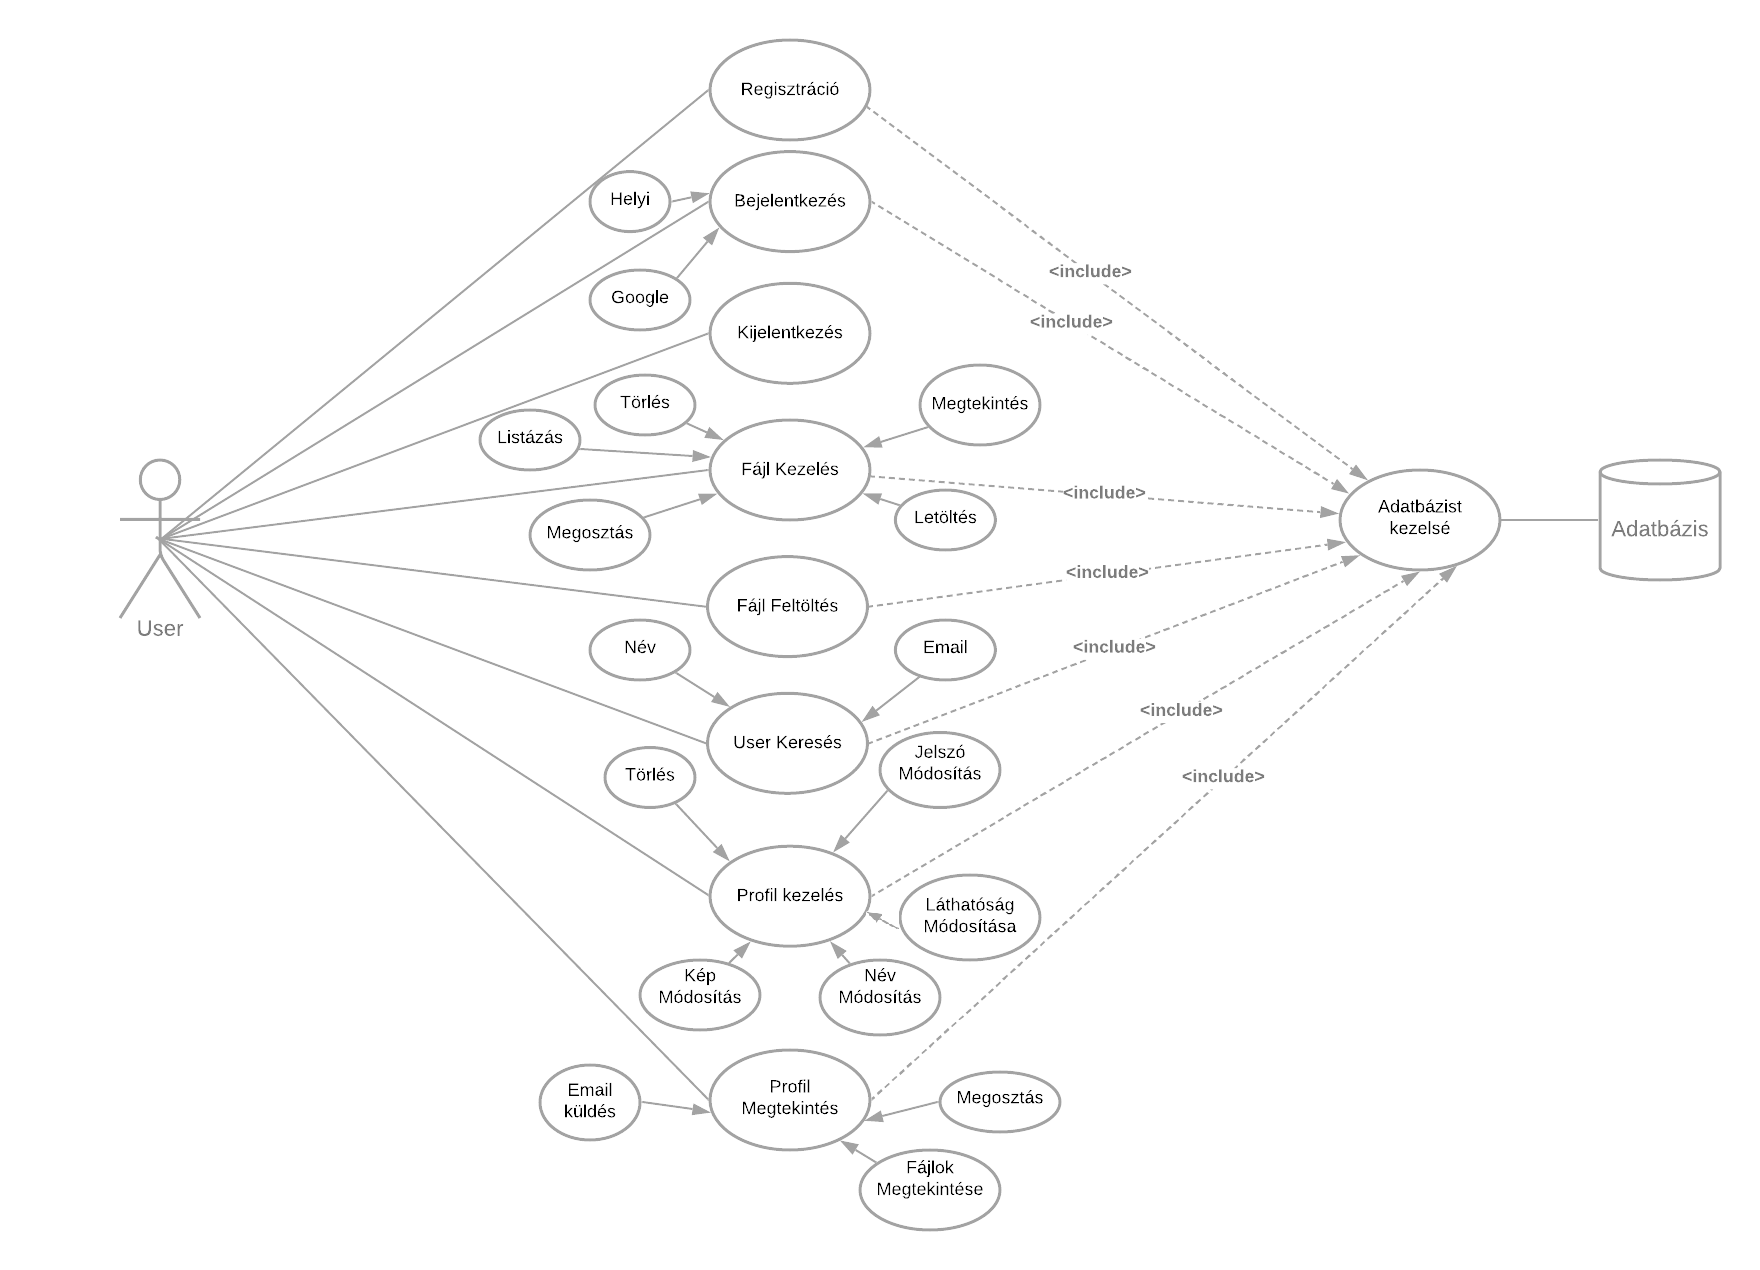
\includegraphics[width=150mm,scale=0.5,]{usecase.png}
\end{center}

A fenti ábrán is látható, hogy az alkalmazás az lényegében adatbázis kezelésre épül. Mivel az applikáció Firebase Firestore adatbázisát használja, ami egy felhő-adatbázis, és minden interakció végrehajtásához ehhez az adatbázishoz intézünk kéréseket, így a szoftver használatához elengedhetetlen az internetkapcsolat megléte az eszközön, amelyen használni szeretnénk azt. Ennek hiányában, a kijelentkezésen kívül, ami lokálisan történik az eszközön, az alkalmazás nem tud kérést indítani, és semmiféle adat nem lesz elérhető.

\subsection{Felhasználó autentikáció}
A ClouDocs alkalmazás használatához első körben a felhasználónak regisztrálnia kell magát. A profil létrehozása elengedhetetlen, mert ez által tudjuk a felhasználók által feltöltött fájlokat elkülöníteni. Amennyiben az applikációt használni kívánó személy mégsem szeretné ezt a lépést végrehajtani, a szoftver lehetőséget biztosít, hogy egy, már létező Google fiókkal jelentkezzünk be, és az újonnan létrejövő profilban az innen beérkező felhasználói adatok kerülnek mentésre. Az alkalmazás elindításakor a szoftver felajánlja a bejelentkezést. Itt a felhasználó a regisztrációnál megadott email cím és jelszó párossal vagy a Google profiljához tartozó bejelentkezési adatokkal férhet hozzá az applikáció többi részéhez. A regisztrációs oldalra a bejelentkezés alatt felkínált opcióval, vagy az oldalsó menüben megjelenő „Sign up” menüponttal lehet eljutni.

\begin{center}
	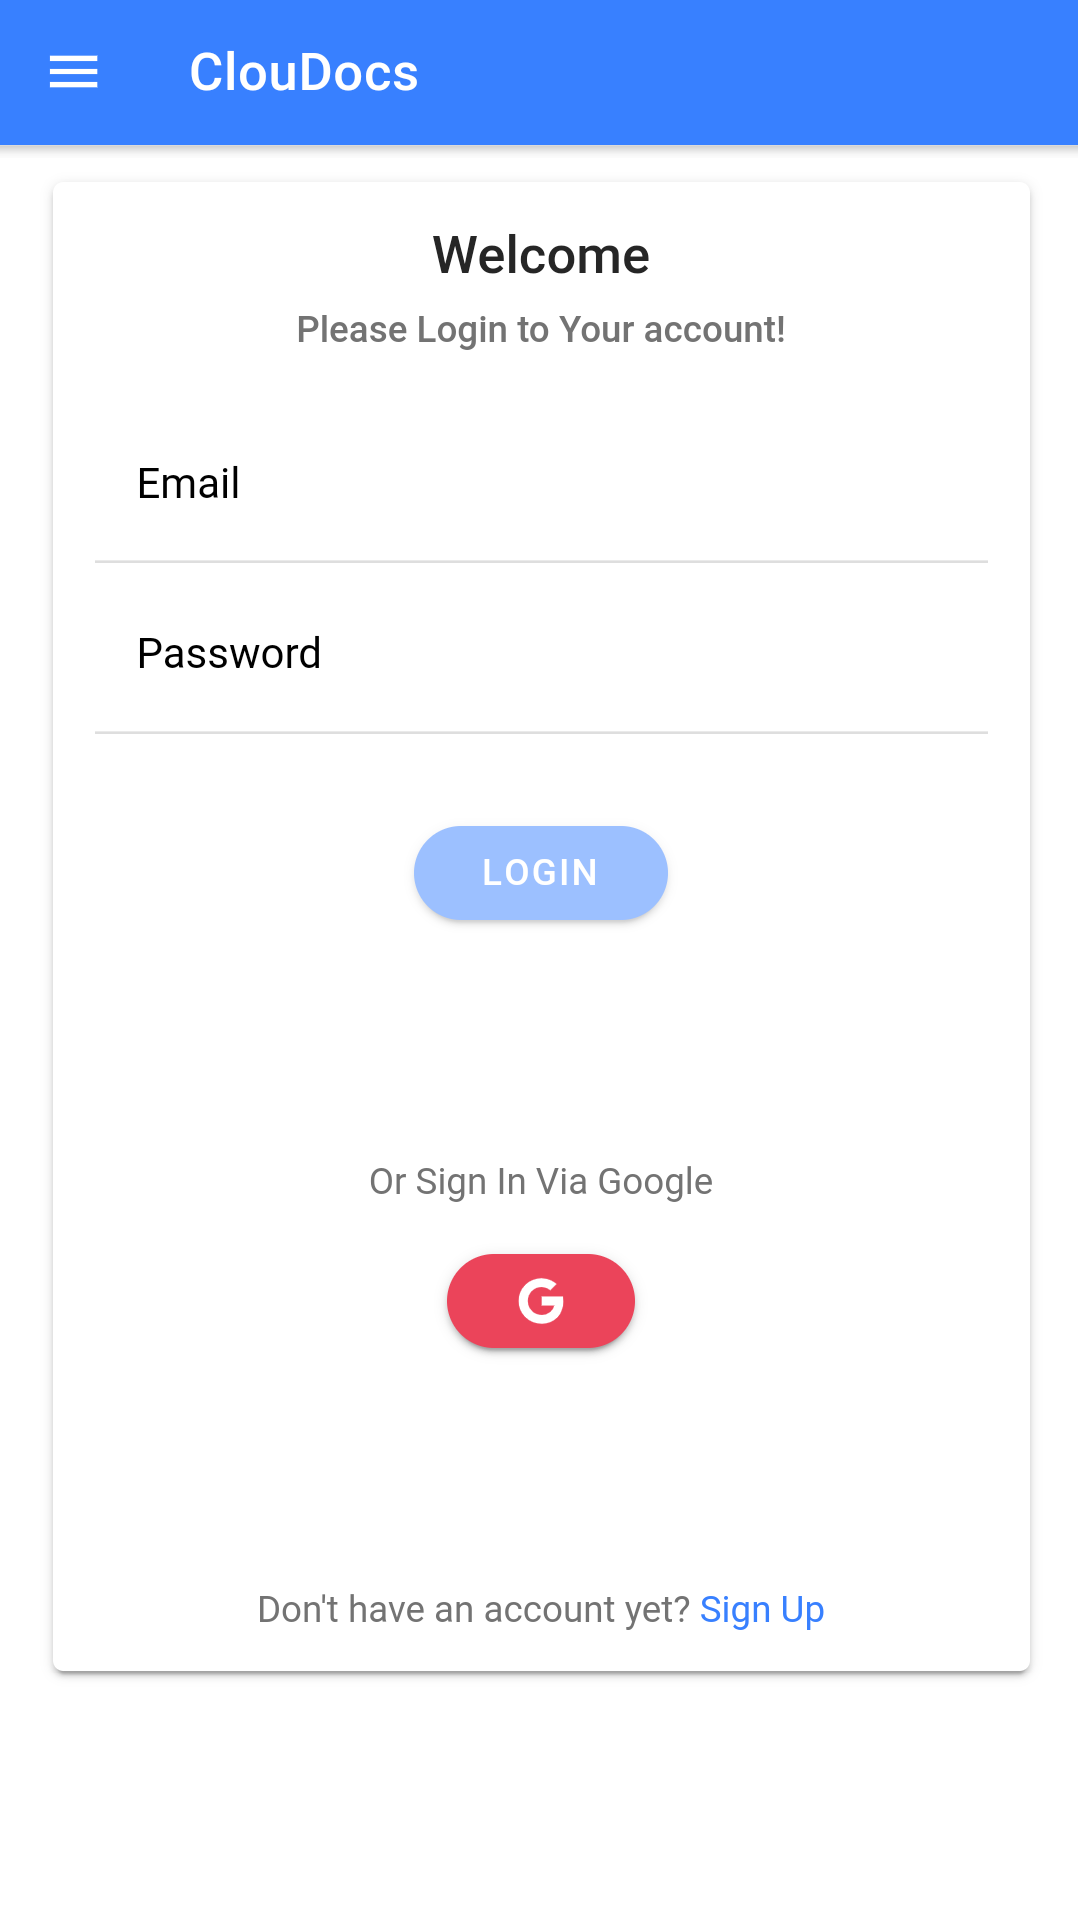
\includegraphics[width=50mm,scale=0.5,]{login.png}
	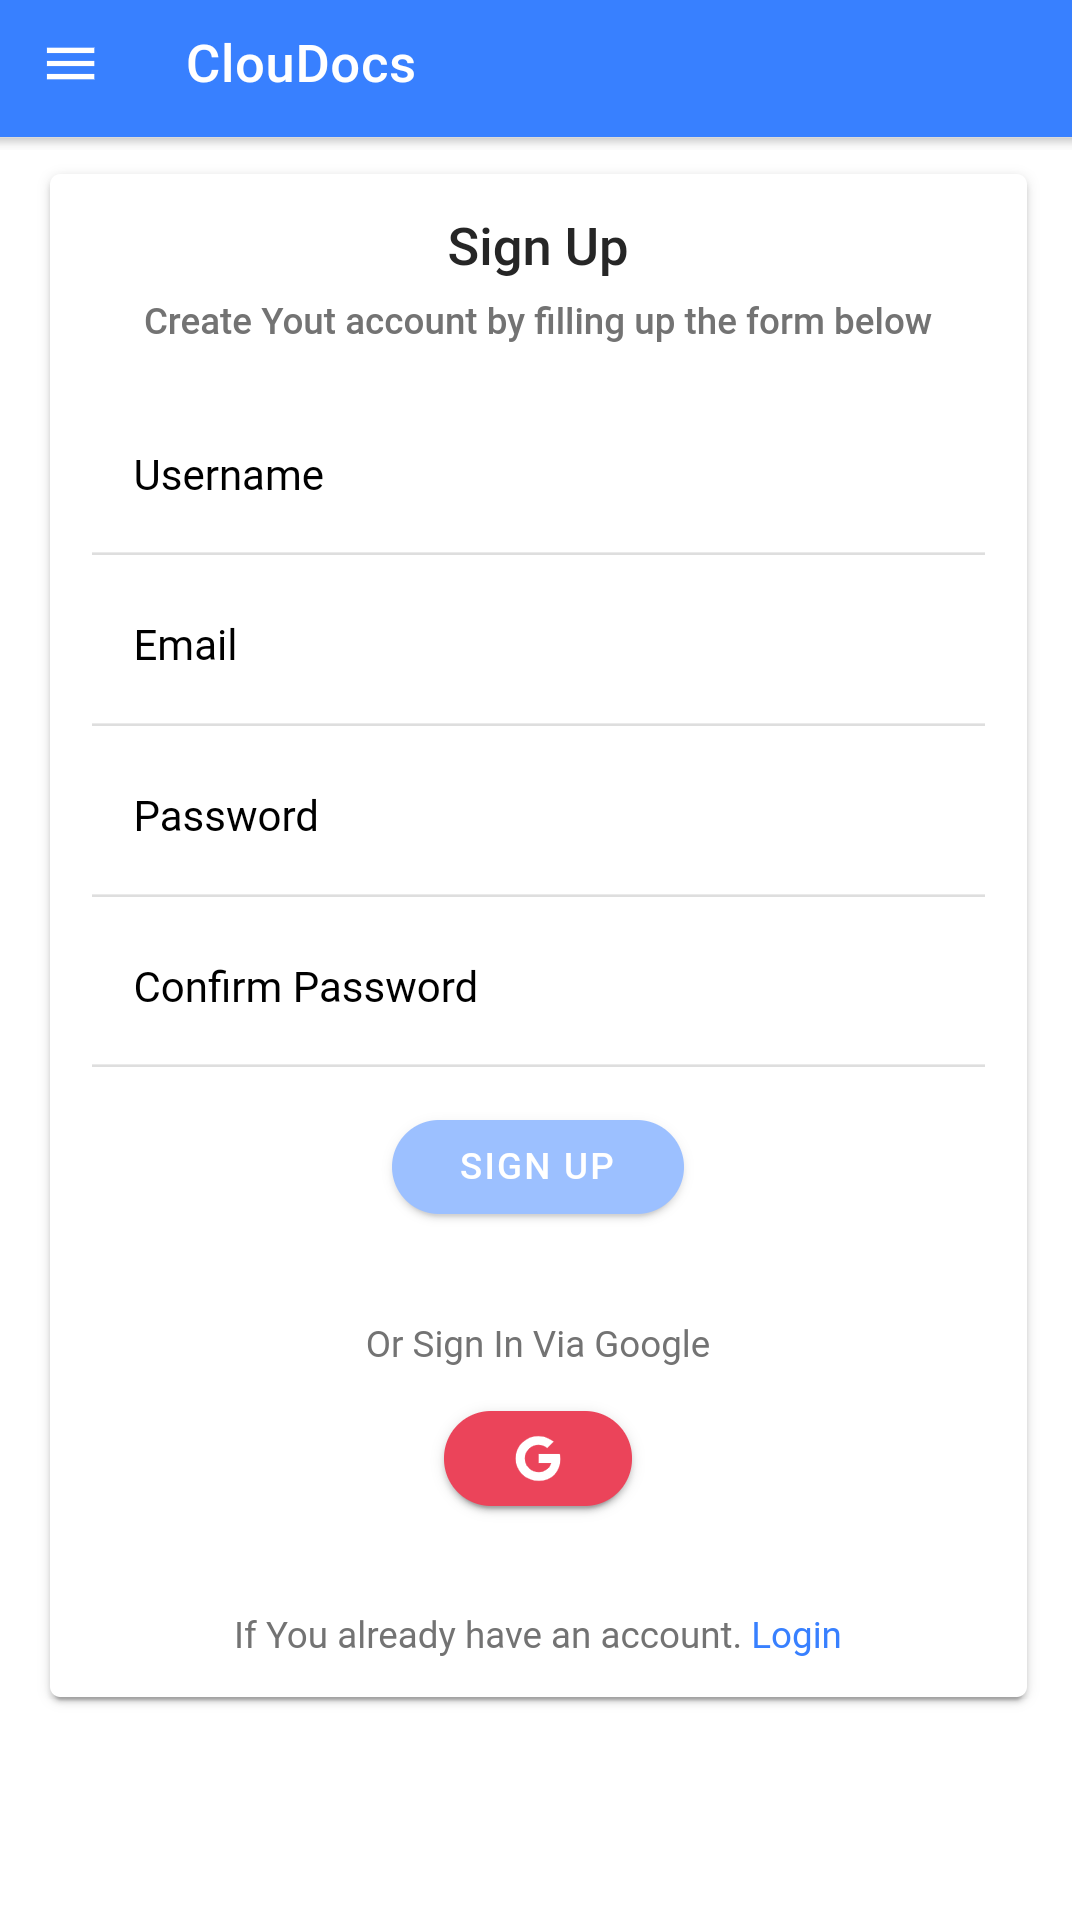
\includegraphics[width=50mm,scale=0.5,]{registration.png}
\end{center}

A regisztráció során, az oldalon megjelenő beviteli mezőkben 3 fontos adatot kell megadniuk a leendő felhasználóknak. Az email címüket, amellyel a későbbiekben a bejelentkezést tudják végrehajtani, más felhasználók ez alapján tudnak rá keresni a profiljukra és az email-en keresztüli kommunikációhoz is szükséges. A felhasználónevüket, mellyel szintén a profiljuk elérhetősége miatt van leginkább szükség. Ez a későbbiekben megváltoztatható és nem egyedi. Legutolsó sorban pedig a jelszavukra, amelyre szintén a bejelentkezés miatt van szükség, és ez is bármikor megváltoztatható. Biztonsági okokból a jelszó kétszeri egymás utáni megadása kötelező a sikeres regisztráció végrehajtásához. Sikeres regisztráció esetén a bejelentkezési adatok létrejönnek, de ekkor még maga a felhasználói profil nem elérhető. A teljes profil létrehozása az adatbázisban az első bejelentkezés alkalmával fog létrejönni, ezzel kiküszöbölve, hogy egy soha nem használt felhasználói profil jöjjön létre és foglalja a tárhelyet.

\subsection{Felhasználó felhő tárhelye}
Sikeres bejelentkezést követően az alkalmazás átirányít minket a tárhelyünket megjelenítő, „Files” oldalra. Itt a már feltöltött fájljainkat és létrehozott mappáinkat tudjuk megtekinteni és interakcióba lépni velük. A tárhelyben lévő mappák mindig a feltöltött fájlok előtt, a lista elején jelennek meg, így megkönnyítve a továbbnavigálást. Egy mappára kattintva a tárhelyünk elemeit tartalmazó lista frissül, a benne lévő elemek a kiválasztott mappa által tartalmazott fájlok és további mappák. A mappák közti visszafelé navigálást a lista elején megjelenő „..” elemmel vihetjük véghez. A mappáinkat továbbá tudjuk törölni, mellyel az összes benne található fájl és almappa is törlődik a tárhelyünkről. A feltöltött fájlokkal a felhasználó, a tárhelyből való eltávolítás mellett, más funkciókat is végrehajthat. Az elemre való kattintással a feltöltött fájl, az eszköz böngészőjének segítségével, megtekinthető. Az elemeket balra húzva jelennek meg a további funkciók. A megosztás gomb megnyomásával a megtekintéshez is használt, a fájlra vezető link másolásra kerül az eszköz vágólapjára, a letöltésre kattintva pedig a lokális tárhelybe menthetjük a kiválasztott elemet. A listában lévő elemeken történő jobbra húzással pedig a már említett törlés funkciót érhetjük el.
\\
\\
\\
Szintén ezen az oldalon tudunk bővíteni a tárhely tartalmát is. Mobil eszközön az oldal bal alsó sarkában megjelenő, úgynevezett „floating action button” (későbbiekben: „fab”) megnyomásával az applikáció két lehetőséget kínál fel a felhasználónak. Létre tud hozni új mappát és feltölthet új fájlokat. Új mappát létrehozni, a leendő mappa nevének megadásával lehet, a feltöltésre kattintva pedig az eszköz lokális tárhelye nyílik meg, ahol a feltölteni kívánt elemre kattintva az el is indul.
\\
\\
\\
A szoftver webes alkalmazásának kinézet itt különbözik leginkább a mobil eszközökön futó natív alkalmazásoktól. Itt a „fab” helyett a felhasználó a két opció közül választhat. A kijelző jobb oldalán lévő, szaggatott vonallal körülhatárolt, úgynevezett „DropZone” mezőbe húzza be a feltölteni kívánt fájlt, vagy a „Fájl kiválasztása” gombra kattintva kiválasztja azt. Itt lehetősége van a felhasználónak egyszerre több elem feltöltését is kezdeményeznie. A mappa létrehozás ebben az esetben az elemeket listázó, a kijelző bal oldalán elhelyezkedő rész, bal felső sarkában megtalálható mappa ikonra kattintva érhető el. Platformtól eltekintve, mindkét funkció végrehajtása során a tárhelybe felkerülő új elem elérési útvonala az éppen aktuálisan kilistázott mappa lesz.

\subsection{Felhasználókeresése}
A „search” oldalon az alkalmazás további regisztrált felhasználói között böngészhetünk. Ezt megtehetjük név- vagy email alapú kereséssel, de a kettőt kombinálni is lehet. A listázott elemek valamelyikére kattintva az ahhoz tartozó felhasználói profilra navigál át minket az alkalmazás. Itt, ha az adott felhasználó profilja nem privát, akkor a neve és email címe mellett a feltöltött fájljai is megtekinthetővé válnak. Ezeket a fájlokat, ahogyan a saját tárhelyünkben, úgy itt is megoszthatjuk vagy letölthetjük. Ha az adott profil, amit meg szeretnénk tekinteni mégis privát, akkor emailben kérhetjük a tulajdonosát ennek átállítására. Lehetőség van továbbá a felhasználói profilok megosztására is, de megtekinteni őket csak bejelentkezés után lehet.

\begin{center}
	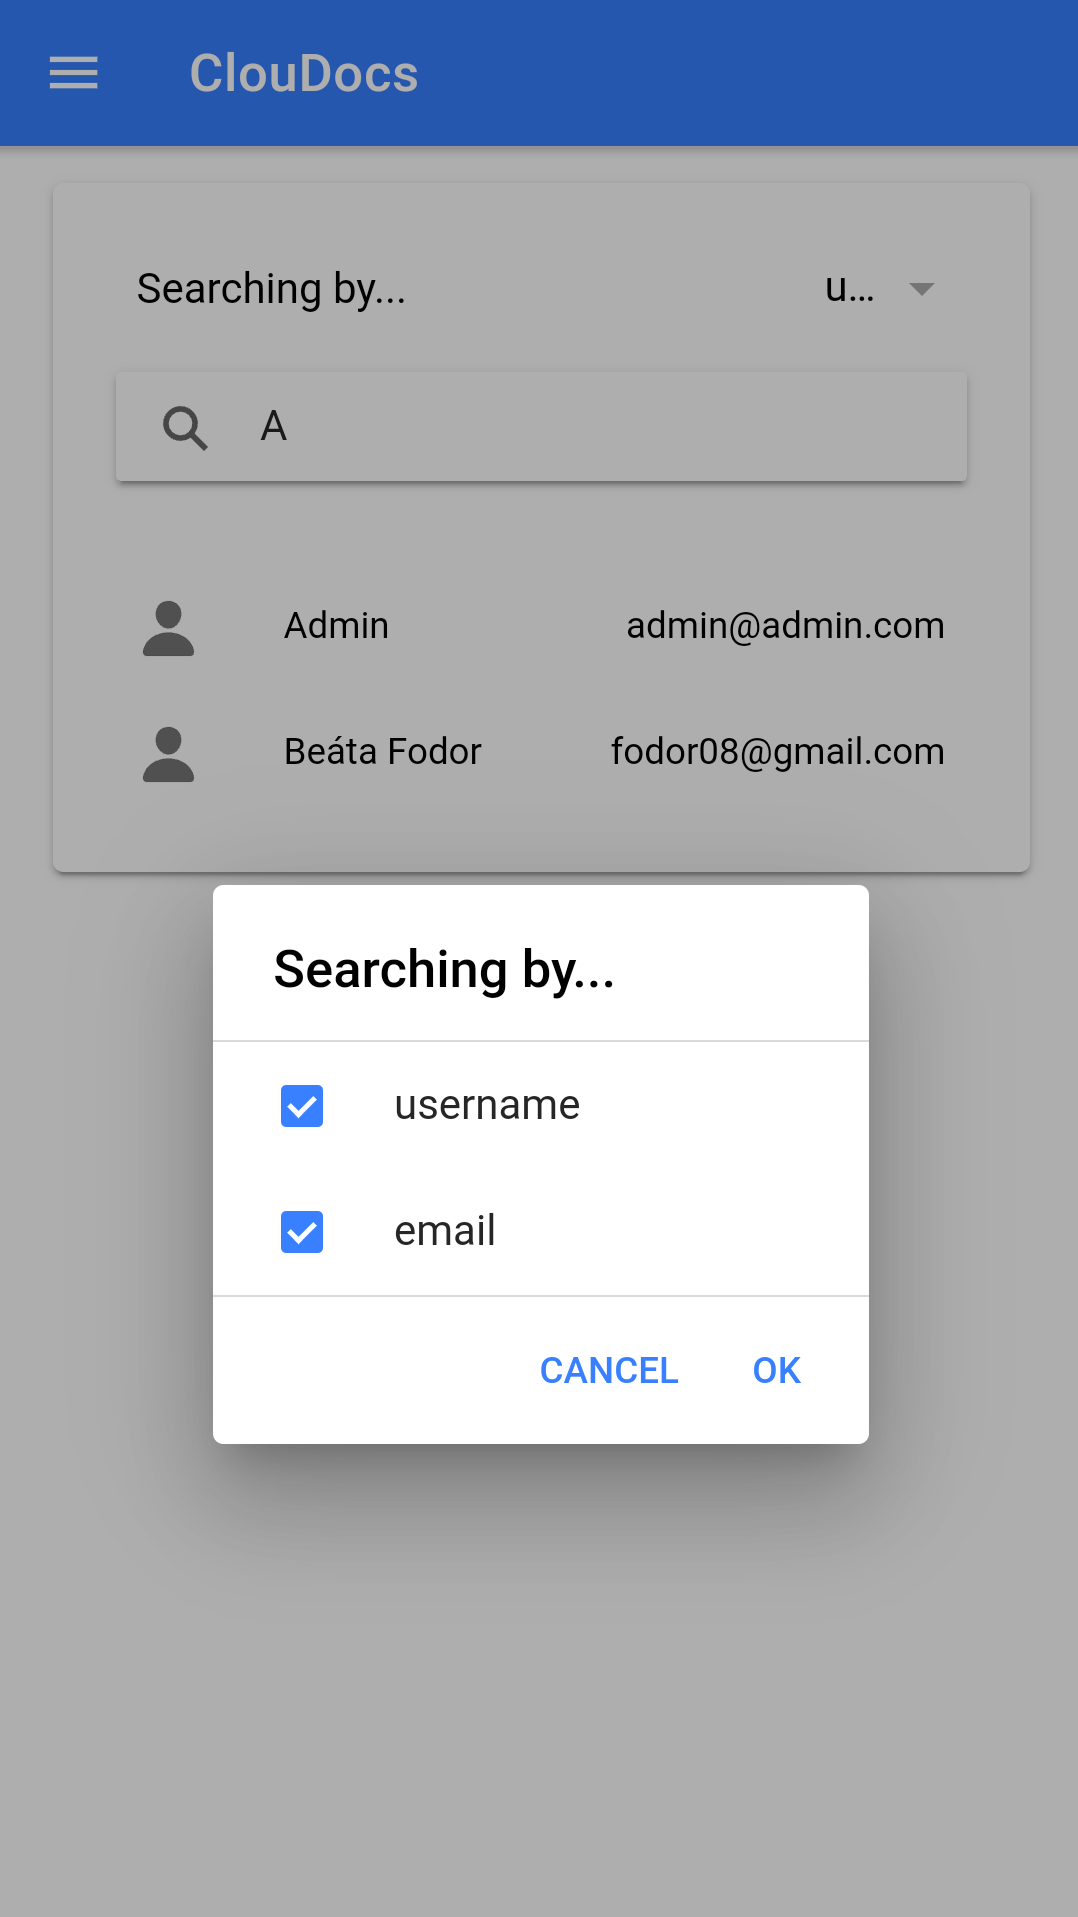
\includegraphics[width=50mm,scale=0.5,]{search.png}
\end{center}

\subsection{Profil menedzsment}
A profil oldalon a felhasználó a saját fiókját tudja kezelni. Pár tájékoztató jellegű információ mellett a fiókhoz tartozó profilképét tudja beállítani vagy frissíteni. Megváltoztathatja a felhasználónevét vagy a bejelentkezéshez szükséges jelszavát, továbbá a profilja láthatóságát is átállíthatja. A láthatóság minden új fiók esetében automatikusan privát, ezt itt a felhasználó maga tudja átállítani, ha láthatóvá szeretné tenni a feltöltött dokumentumait más regisztrált személyek számára. Emellett lehetőség van a fiók törlésére is, mellyel minden feltöltött fájl is törlésre kerül.

\section{Szerkezeti felépítés}
Az Angular keretrendszer egyik fő előnye, hogy szerkezeti sajátosságából adódóan, az üzleti logikát és a kinézetért felelős kódrészleteket külön lehet választani, amivel struktúráltabb forráskódot kapunk. A keretrendszer alapjai a modulok és azok komponensei, szolgáltatásai, de lehetőséget nyújt saját direktívák, interfészek és úgynevezett csövek létrehozására is.\\
Az alábbiakban az általam fejlesztett alkalmazás szerkezeti felépítését, modulokra, komponensekre és szolgáltatásokra bontva mutatom be.

\subsection{Modulok}
Az Angular keretrendszerrel fejlesztett alkalmazások úgynevezett NgModulokat használnak. Ezek minden esetben egy „@NgModule” dekorátorral ellátott osztályok, mely segít azonosítani a modul saját komponenseit, direktíváit és csöveit, továbbá a modul által használt különböző szolgáltatások injektálásai is itt adhatók meg. Az NgModulok sajátossága továbbá, hogy a modulok használhatják az egymás által exportált funkcióikat is.\\
A ClouDocs-ban az alkalmazás gyökérmodulján (AppModule) kívül, minden oldal saját modullal rendelkezik. Ezekben a modulokban az oldalak egyszerűbb funkciói kaptak helyet, elsősorban az oldalakon megjelenő gombok kezeléséért, vagy a megjelenő tartalomért felelős metódusok. Továbbá az AppRoutingModule felelős az alkalmazáson belüli navigálásért. Az alkalmazás által használt modulok név szerint a következők:
\begin{itemize}
	\item AppModule
	\item AppRoutingModule
	\item HomePageModule
	\item LoginPageModule
	\item RegistrationPageModule
	\item FilePageModule
	\item ProfilePageModule
	\item SearchPageModule
	\item UserPageModule
\end{itemize}

\subsection{Szolgáltatások}
A szolgáltatások fő célja, hogy a bennük implementált metódusokat, az ott létrehozott változókat és adatokat az alkalmazás különböző moduljai elérhessék és használhassák. Egy Angular projekten belül a szolgáltatások a felelősek a megjelenítésért és az üzleti logikáért felelős kódrészek elkülönítéséért. Az alkalmazás moduljai és komponensei helyett, a kifejezetten működést megvalósító kódok kiszervezhetőek a szolgáltatásokba, így megvalósítva a szeparációt és megkönnyítve a fejlesztést.\\
A ClouDocs alkalmazásban több kisebb és nagyobb szolgáltatás került implementálásra. A következőkben ezeket és a fontosabb metódusaikat mutatom be röviden.

\subsubsection{AuthService}
Ebben a szolgáltatásban az autentikációért felelős kódrészletek és a Firebase Authentication felhő-szolgáltatásával való kommunikáció van megvalósítva.

\begin{itemize}
	\item login(u): ez a metódus a kapott paraméter segítségével, ami egy email- és jelszó párossal rendelkező felhasználó objektum, elvégzi a felhasználó bejelentkeztetését, ha az egy helyi fiókkal történik.
	\item GoogleAuth(): ez a metódus felelős a Google fiókkal való bejelentkezésért mind a web- mind a natív alkalmazásban.
	\item signUp(u): ez a kódrészlet felelős a sikeres regisztrációt követően, a kapott paraméter alapján, a bejelentkezési adatok létrehozásáért.
	\item signOut(): itt van megvalósítva a kijelentkezés, mely a Firebase Authentication-ből való kijelentkeztetés után a lokális tárhelyből is eltávolítja a fiókhoz tartozó id-t.
\end{itemize}

Ezek mellett még tartalmazza pár adat „getter-setter” metódusait, a fejlesztés megkönnyítése érdekében.

\subsubsection{LoginService}
Ez a szolgáltatás valósítja meg az AuthServiceben történt bejelentekzést követően a felhasználó tárolását a Firebase Firestore adatbázisában tárolt „profiles” kollekcióba.

\begin{itemize}
	\item saveUser(res): a bejelentkezést követően a kapott adatokból a felhasználó adataival létrehoz a Firestore-ban egy dokumentumot az említett „profiles collectionbe”, abban az esetben, ha ez a dokumentum még nem létezne. Emellett az alkalmazáson belül is elmentésre kerülnek ezek az adatok. Továbbá a bejelentkezett felhasználó id-ját elmenti a lokális tárhelybe, ezzel megkönnyítve a bejelentkezés utáni, a navigáció végrehajtásához szükséges autentikációs folyamatokat.
	\item login(u) és GoogleLogin(): a bejelentkezés végrehajtásával kapott eredményeket továbbítják paraméterül átadva a „saveUser” metódus meghívásakor.
\end{itemize}

\subsubsection{ManageService}
Ez a szolgáltatás a feltöltött fájlok kezelését megvalósító funkciókat tartalmazza és ezekhez a Firebase Storage felsző-szolgáltatásával kommunikál.

\begin{itemize}
	\item delete(f): ez a metódus a paraméterül kapott fájl vagy mappa törlését implementálja. Ha a kapott paraméter fájl, csak törli azt a Firebase Storage-ból. Abban az esteben viszont, ha egy mappát kap, akkor rekurzív hívás segítségével törli a benne lévő összes fájlt, és ez által a mappákat is.
	\item createFolder(aF): ez a kódrészlet valósítja meg az új mappa létrehozását a tárhelyben. Ehhez paraméterül kapja a tárhely aktuális mappájának elérési útvonalát, és ott hozza létre a felhasználó által megadott néven.
	\item shareNative(f, url): natív alkalmazásban a vágólapra való másoláshoz külön csomagot kell használni. Ez a metódus a csomag „copy” funkcióját meghívva kimásolja a paraméterül kapott publikus fájl url-jét, majd egy úgynevezett „Toaster Message” fomájában erről értesíti a felhasználót is.
\end{itemize}

A feltöltött fájlokkal megvalósítható interakcióba tartozik még a letöltés is. Viszont ez a funkció, az összetettségéből adódóan külön szolgáltatásban lett megvalósítva.

\subsubsection{DownloadService}
Egyetlen metódusa a downloadFile(), mely... \\
\\
\\
\\

\subsubsection{UploadService}
A ClouDocs alkalmazás legösszetettebb szolgáltatása. Mivel a szoftver elsődlegesen a fájlok feltöltésének megvalósítására jött létre, így ez a szolgáltatás a leghangsúlyosabb mindközül.

\begin{itemize}
	\item chooseFile(): a natív alkalmazáson belüli fájlfeltöltéshez a FileChooser nevű Cordova plugin „open” metódusát hívja meg, az így kapott „file urit” továbbítja a „makeFileIntoBlob()” függvénynek, amely segítségével már egy feltölthető állományt kapunk. A feltöltés is itt hívódik meg.
	\item choosePhoto(): ugyanúgy működik, mint az előbb bemutatott  „chooseFile” metódus, annyi korlátozással, hogy a csak képfájl tölthető fel vele. Ez valósítja meg a felhasználó profilképének cseréjekor történő fotófeltöltést.
	\item  getFileType(): ez a metódus a „makeFileIntoBlob” során hívódik meg, és a fájlnév alapján, ami tartalmazza a fájl kiterjesztésést is, visszatér a kiterjestés alapján a fájl úgynevezett „mime typejával”.
	\item  uploadToFirebasePhoto() és uploadToFirebasePhotoWeb(): függvényhívások tekintetében itt is különbözik a web- és a natív alkalmazás, így külön metódusokban, de egyazon funkció megvalósítására íródtak. Segítségével a felhasználó a fiókjához tartozó profilkép lecserélésekor a fotót feltölti a Firebase Storage egy külön mappájába, ami a felhasználók számára nem elérhető, majd a képhez tartozó url címét frissíti a Firestore felhasználóhoz tartozó dokumentumában.
	\item 	uploadBlobToFirebase() és uploadBlobToFirebaseWeb(): itt is a függvényhívások és paraméterátadások miatt volt szükség két külön metódusra egy funkció megvalósításához. Itt a paraméterben kapott fájl blob feltöltése van megvalósítva a Firebase Storage-ba. A feltöltés folyamata valós időben eltárolódik, így megjeleníthető a felhasználó számára az előrehaladás, a folyamat esetleges megállása esetén pedig a tárolt adatok alapján a feltöltés folytatható. Az utolsó blob feltöltését követően a fájl adataival létrejön egy új dokumentum a Firestore „files” nevű kollekciójába.
	\item isActive(): visszatér egy boolean értékkel, hogy a feltöltés folyamata aktív-e.
	\item isDone(): szintén boolean értékkel visszatérő metódus, ami azt mutatja, hogy a feltöltési folyamat befejeződött-e.
\end{itemize}

\subsubsection{ChunkService}
A DownloadService-hez hasonlóan szintén az összetettsége miatt külön szolgáltatásba szerveztem ki a feltöltéskor a fájlok felbontását végző metódust.

\begin{itemize}
	\item calculateSize(): a parméterül kapott fájlt felbontja 10Mb méretű részekre, úgynevezett „chunkokra”, majd mindegyikre egyesével hívja meg az UploadService-ben található feltöltést megvalósító függvényt.
\end{itemize}

Ezekben a szolgáltatásokban lettek megvalósítva az alkalmazás lényeges funkcióinak működéséhez szükséges és azokat megvalósító metódusok. Ezek mellett viszont még helyet kaptak kisebb, 1-1 segédfunkciókat megvalósító szolgáltatások. Ezeket csak említés szintjén szeretném bemutatni.

\begin{itemize}
	\item PlatformSevice: getter-setter metódusokat tartalmazó szolgáltatás, mellyel megkapható az aktuális eszköz platformja, amelyen az alkalmazás fut.
	\item NotificationsService: a web alkalmazáson belüli értesítések megjelenítéséhez használandó metódusokat tartalmaz.
\end{itemize}

\subsection{Alkalmazáson belüli navigáció - Routing}
Az Angular keretrendszert használó alkalmazások úgynevezett „Single Page Application”-ök (SPA). Esetükben a navigáció során nem töltődnek be új fájlok, csak az alkalmazás indulásakor betöltött egyetlen fájljának tartalma változik. Ezt a moduloknál is említett AppRoutingModule valósítja meg.\\
Az AppRoutingModule-ban definiálva van az összes oldal modulja és a hozzájuk tartozó elérési útvonalak (url-ek) is. Ezáltal, amikor egy oldalra navigálunk, akkor a navigáció során a céloldal url-je alapján az AppRoutingModule betölti a hozzá tartozó oldal modulját, ami tartalmazza a kinézetért felelős html és a funkciók megvalósításáért felelős fájlokat. Az alábbi ábrán az általam készített alkalmazás routing-ját szemléltető ábrája látható.\\
\\
\\
\\
Az alkalmazás indításakor minden esetben a gyökér elérési útvonalhoz tartozó oldal modulja jelenik meg. Ez a ClouDocs alkalmazásban a HomePageModul. A különböző útvonalakhoz rendelhetünk akár úgynevezett „guardokat” is, melyek megakadályozzák az illetéktelenek hozzáférését bizonyos oldalahoz. Ebben az alkalmazásban a FilePageModule, a SearchPageModule és a ProfilePageModule van ilyen módon védve. Az AuthGuard osztály definiál egy szabályt, ami „false” értékkel tér vissza, ha a lokális tárhelyben nem talál bejelentkezett felhasználót, így megtagadva a nem-bejelentkezett személytől ezen oldalak megtekintését. A ClouDocs-ban a navigálást a minden oldalon megjelenő SidebarComponent oldalsó navigációs menüvel valósíthatja meg a felhasználó. Ennek tartalma dinamikusan változik a be- és kijelentkezés során. Ezzel is elősegítve a privát oldalak védelmét. Ebben az alkalmazásban nincsenek összetett url címek. Egyedül egy másik felhasználó profiljának megtekintésekor jön létre egy egyszeresen összetett elérési útvonal, ahol „/users” után a megtekintett felhasználó saját id-ja szerepe. Ennek az útvonalnak a segítségével tudja az alkalmazás a megfelelő felhasználói adatokat betölteni.


\end{document}